\documentclass[conference, a4paper]{IEEEtran}
\IEEEoverridecommandlockouts

\usepackage{lipsum}
\usepackage{url}
\usepackage{graphicx}
\usepackage[caption=false, font=footnotesize]{subfig}

\usepackage{glossaries-prefix}
\usepackage{tabularx}
\usepackage{amsmath}

\makeglossaries
\newacronym[prefixfirst={a\ },prefix={a\ }]{dl}{DL}{deep learning}

\newcommand\figref{Fig.~\ref}
\newcommand\figsref{Figs.~\ref}

\begin{document}

% ============ 1 =======================
\title{Your Title}

\author{
\IEEEauthorblockN{First Author}
\IEEEauthorblockA{
\textit{Computer Science Department},\\ \textit{Faculty of Computing and Media}, \\
Bina Nusantara University, \\
Jakarta, Indonesia 11480\\
first.author@binus.ac.id}
\and
\IEEEauthorblockN{Second Author}
\IEEEauthorblockA{
\textit{Computer Science Department},\\ \textit{Faculty of Computing and Media}, \\
Bina Nusantara University, \\
Jakarta, Indonesia 11480\\
second.author@binus.ac.id}
\and
}

\maketitle

% ============ 1 =======================

% ============ 2 =======================
\begin{abstract}
\boldmath 
\lipsum[1]
\end{abstract}

\begin{IEEEkeywords}
keyword1, keyword2.
\end{IEEEkeywords}

% ============ 2 =======================

% ============ 3 =======================
\section{Section Title}
\label{sec:title}

Write something before a subsection. 
In Section~\ref{sec:title}, we will discuss. 

\subsection{Subsection Title}
\label{sec:sub:title}

\Gls{dl} is an extension of multilayer perceptron.

\lipsum[1-2]

% ============ 3 =======================

% ============ 4 =======================
\section{Citation}
\label{sec:citation}

You can cite a paper this way \cite{lecun2015deep}. 
Find more examples on the official IEEETran website\footnote{\url{http://tug.ctan.org/biblio/bibtex/contrib/IEEEtran/IEEEexample.bib}}.  

\lipsum[1]

% ============ 4 =======================

% ============ 5 =======================
\section{Figures}
\label{sec:figures}

Make sure that all figure labels should be referred in the main text.
For example, Fig.~\ref{fig:figure1} is an example of referring an individual image in the main text.
I also added a custom command such that you can refer a figure this way, i.e., \figref{fig:figure1}.
Fig.~\ref{fig:figure4x1} depicts a way to show multiple images within a figure environment.
You could refer it individually this way, e.g., Fig.~(\ref{1a}).


    \begin{figure}[]
      \begin{center}{}
          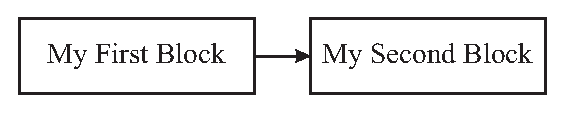
\includegraphics[width=1\columnwidth,draft=false]{./figs/figure1.eps}
          \caption{14pt.}
          \label{fig:figure1}
      \end{center}
    \end{figure}

    \begin{figure}[]
        \centering
      \subfloat[14pt\label{1a}]{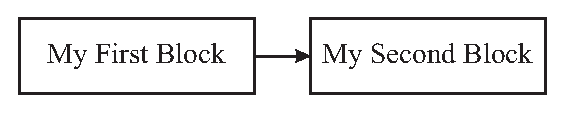
\includegraphics[width=1\columnwidth]{./figs/figure1.eps}}
      \\
      \subfloat[12pt\label{1b}]{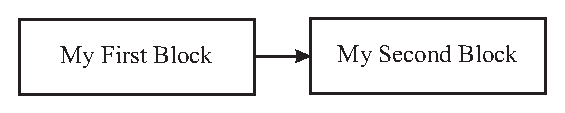
\includegraphics[width=1\columnwidth]{./figs/figure2.eps}}
        \\
      \subfloat[10pt\label{1c}]{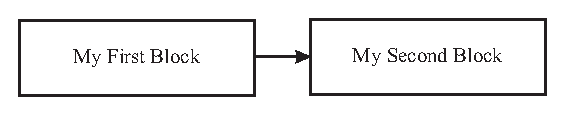
\includegraphics[width=1\columnwidth]{./figs/figure3.eps}}
        \\\
      \subfloat[8pt\label{1d}]{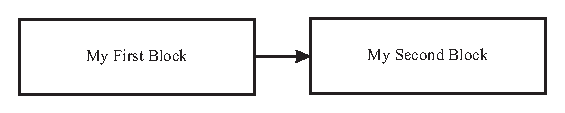
\includegraphics[width=1\columnwidth]{./figs/figure4.eps}}
      \caption{(a), (b), (c), (d).}
      \label{fig:figure4x1} 
    \end{figure}
    
    \begin{figure*}[]
      \begin{center}{}
          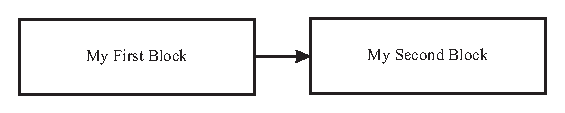
\includegraphics[width=2\columnwidth,draft=false]{./figs/figure4.eps}
          \caption{8pt.}
          \label{fig:figurefull}
      \end{center}
    \end{figure*}


% ============ 5 =======================


% ============ 6 =======================
\section{Tables}
\label{sec:tables}

Also, do not forget to refer tables that are included in an academic paper, e.g., Table~\ref{tab:basic}

\begin{table}[]
\centering
\caption{A very basic table}
\label{tab:basic}
\begin{tabular}{|l|l|l|l|l|}
\hline
a & b & b & d & e \\ \hline
1 & 2 &   &   &   \\ \hline
  &   &   &   &   \\ \hline
  &   &   &   &   \\ \hline
\end{tabular}
\end{table}

\begin{table}[]
\centering
\caption{A very multicolumn table}
\label{tab:multicolumn}
\begin{tabular}{|ll|l|l|l|}
\hline
\multicolumn{2}{|c|}{a}     & b & d & e \\ \hline
\multicolumn{1}{|l|}{1} & 2 &   &   &   \\ \hline
\multicolumn{1}{|l|}{}  &   &   &   &   \\ \hline
\multicolumn{1}{|l|}{}  &   &   &   &   \\ \hline
\end{tabular}
\end{table}

\begin{table}[]
\centering
\caption{A tabularx table}
\label{tab:tabularx}
\begin{tabularx}{\columnwidth}{|X|l|l|l|l|}
\hline
a & b & b & d & e \\ \hline
1 & 2 &   &   &   \\ \hline
  &   &   &   &   \\ \hline
  &   &   &   &   \\ \hline
\end{tabularx}
\end{table}

% ============ 6 =======================

% ============ 7 =======================
\section{Equations}
\label{sec:eq}

You can do an inline equation like this $y = mx + c$.

    \begin{align}\label{eq:elementalobject}
      \varepsilon = \left\{ \mathbf{p}, \mathbf{n}, m, A, \Psi_\text{c}, R \right\},
    \end{align}
    
    \begin{align*}
      E = mc^2
    \end{align*}

    \begin{align*}
      \log xy = \log x + \log y
    \end{align*}
    
    \begin{align*}
      H = - \sum_i p(x_i) \log p(x_i)
    \end{align*}
    
    \begin{align*}
      v = \frac{x}{y}
    \end{align*}

% ============ 7 =======================


% ============ 8 =======================
\section{Conclusions}
\label{sec:conclusion}

\lipsum[3]


% ============ 8 =======================

\section*{Acknowledgment}
This work is supported by Research and Technology Transfer Office of Bina Nusantara (Binus) University as a part of

\bibliographystyle{IEEEtran}
\bibliography{references}

\end{document}
